\documentclass[a4,12pt]{article}
\usepackage{colortbl}
\usepackage{pgfplots}
\usepackage[margin=2cm]{geometry}
\pgfplotsset{compat=newest}
\begin{document}
\begin{table}
\footnotesize
\sffamily
\begin{center}
\begin{tabular}{cccccccc}
Mean-Accuracy & \shortstack{MultiROCKET \\ 0.8666} & \shortstack{InceptionTime \\ 0.8353} & \shortstack{DefFCN \\ 0.8227} & \shortstack{Inception \\ 0.8097} & \shortstack{FCN \\ 0.8025} & \shortstack{ResNet \\ 0.7738} \\[1ex]
\shortstack{DefFCN \\ 0.8227} & \bfseries \cellcolor[rgb]{0.3837,0.5102,0.9178}\shortstack{\rule{0em}{3ex} -0.0439 \\ 25 / 6 / 81 \\  $\leq$ 1e-04} & \cellcolor[rgb]{0.7438,0.8251,0.9658}\shortstack{\rule{0em}{3ex} -0.0126 \\ 47 / 5 / 60 \\ 0.1360} & \cellcolor[rgb]{0.8674,0.8644,0.8626}\shortstack{\rule{0em}{3ex} Mean-Difference \\ r$>$c / r=c / r$<$c \\ Wilcoxon p-value} & \bfseries \cellcolor[rgb]{0.9528,0.783,0.6986}\shortstack{\rule{0em}{3ex} 0.0130 \\ 74 / 2 / 36 \\ 0.0035} & \bfseries \cellcolor[rgb]{0.9689,0.7108,0.5999}\shortstack{\rule{0em}{3ex} 0.0202 \\ 65 / 3 / 44 \\ 0.0177} & \bfseries \cellcolor[rgb]{0.8204,0.2868,0.2452}\shortstack{\rule{0em}{3ex} 0.0489 \\ 77 / 6 / 29 \\  $\leq$ 1e-04} \\[1ex]
\end{tabular}\\
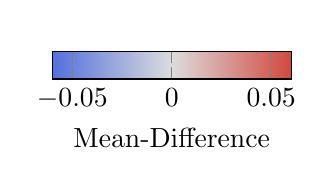
\begin{tikzpicture}[baseline=(current bounding box.center)]\begin{axis}[hide axis,scale only axis,width=0sp,height=0sp,colorbar horizontal,colorbar style={width=0.25\linewidth,colormap={cm}{rgb255(1)=(83,112,221) rgb255(2)=(220,220,220) rgb255(3)=(209,73,62)},colorbar horizontal,point meta min=-0.06,point meta max=0.06,colorbar/width=1.0em,scaled x ticks=false,xticklabel style={/pgf/number format/fixed,/pgf/number format/precision=3},xlabel={Mean-Difference},}] \addplot[draw=none] {0};\end{axis}\end{tikzpicture}\end{center}
\caption{[...] \textbf{If in bold, then p-value $<$ 0.05} [...]}
\end{table}
\end{document}
